\documentclass[14pt,fleqn]{extarticle}
\RequirePackage{prepwell}
\previewoff
\begin{document}

\newcommand\lone{2x+y=4}
\newcommand\ltwo{3x-2y = 6}
\newcommand\lthree{x-3y+5=0}

%text
Using the method of integration, find the 
area of the region bounded by the lines 
\[\lone, \ltwo  \text{ and }  \lthree \]
%

\newcard 

Let us re-write the equations of the lines so that we can eventually plot them 

\begin{align}
	L_1: \lone \implies y &= -2x + 4 \\ 
	L_2 : \ltwo \implies y &= \frac{3}{2}x + 3 \\ 
	L_3: \lthree \implies y &= \frac{x}{3} + \frac{5}{3}
\end{align}

For the three lines, we can see that 
\begin{center}
  \begin{tabular}{NNNN}
  \toprule 
        \text{Line} & \text{Slope }(m) & \text{$x$ intercept} & \text{$y$ intercept}  \\
   \midrule 
   L_1 & -2 & (2,0) & (0,4) \\ 
    \midrule 
    L_2 & \frac{3}{2} & (2,0) & (0,-3) \\ 
    \midrule 
    L_3 & \frac{1}{3} & (-5,0) & \left(0,\frac{5}{3} \right)\\
    \bottomrule
  \end{tabular}
  
\end{center}

Hence, this is how they must look 
\begin{center}
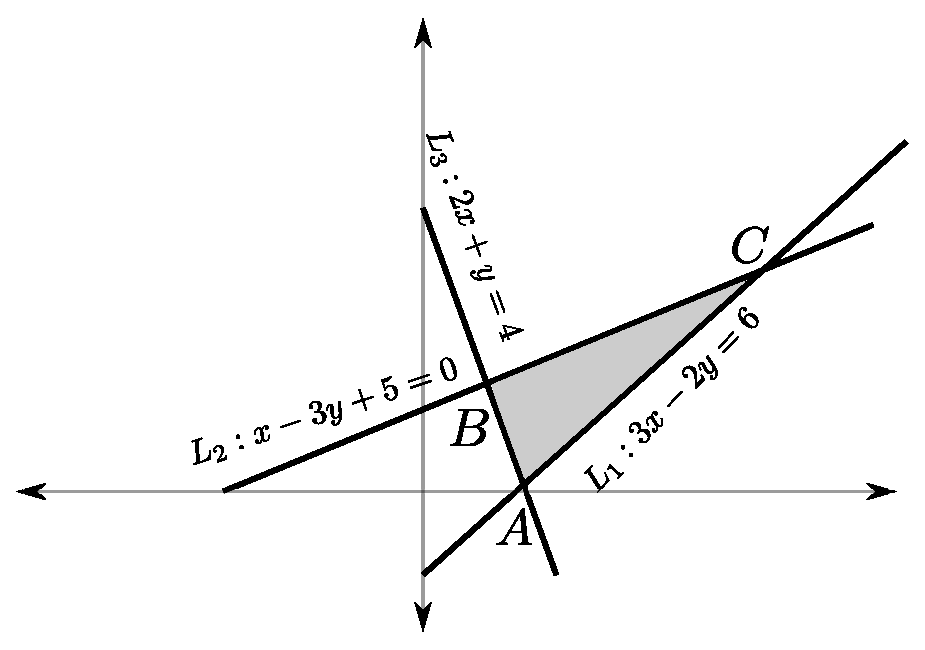
\includegraphics[scale=0.55]{right.eps} 
\end{center} 

\newcard 

\begin{center}
  \begin{tabular}{NN}
  \toprule 
       \text{Pt. of intersection} & \text{Coordinates} \\
   \midrule
   A & \left(2,0 \right) \\
   \midrule
   B & \left(1,2 \right)\\
    \midrule 
    C & \left(4,3 \right) \\
    \bottomrule
  \end{tabular}
\end{center}

\newcard 

\begin{center}
  \begin{tabular}{NN}
  \toprule 
       \text{Pt. of intersection} & \text{Coordinates} \\
   \midrule
   A & \left(2,0 \right) \\
   \midrule
   B & \left(1,1 \right)\\
    \midrule 
    C & \left(5,2 \right) \\
    \bottomrule
  \end{tabular}
\end{center}
\newcard 

We need to find the points of intersection -- $A,B$ and $C$ -- of the three lines \newline 

 Hence, we take two lines at a time and solve for $x$ and $y$ 

\begin{align}
A: y=4-2x &= \frac{3x}{2}-3\implies x = 2, y = 0 \\
B: y=4-2x &= \frac{x}{3}+\frac{5}{3} \implies x = 1, y = 2 \\
C: y = \frac{x}{3}+\frac{5}{3} &= \frac{3x}{2}-3 \implies x = 4,y=3 
\end{align}

\newcard 

The required area $R$ is therefore 
\small\[R = \int_1^4 \frac{x+5}{3}dx - \int_1^2 (4-2x)\cdot dx - \int_2^4 \left( \frac{3x}{2}-3\right)dx\]\normalsize 

\newcard 

Refer back to the diagram again and you will see 

\begin{align}
R &= \underbrace{\text{Area under BC}}_{\text{From B to C}} = \int_1^4 \frac{x+5}{3}dx\\
&- \underbrace{\text{Area under BA}}_{\text{From B to A}}=\int_1^2 (4-2x)\cdot dx \\ 
&- \underbrace{\text{Area under AC}}_{\text{From A to C}}=\int_2^4 \left( \frac{3x}{2}-3\right)dx
\end{align}\newline 

And so we get the expression 
\small\[R = \int_1^4 \frac{x+5}{3}dx - \int_1^2 (4-2x)\cdot dx - \int_2^4 \left( \frac{3x}{2}-3\right)dx\]\normalsize 

\newcard 

\[ \qquad R = \frac{7}{2}\]

\newcard 

\[ \qquad R = \frac{5}{2}\]

\newcard 

The following standard result has been applied in the calculations below \[\qquad\qquad \int x^n\cdot dx = \frac{x^{n+1}}{n+1}\]

Which gives us 

\begin{align} 
R &= \left[ \int_1^4 \frac{x+5}{3}dx =\frac{1}{3}\left[ \frac{x^2}{2} + 5x \right]_1^4 = \frac{15}{2}\right]\\ 
&- \left[\int_1^2 (4-2x)\cdot dx = \left[ 4x-x^2\right]_1^2 = 1 \right]\\
&- \left[\int_2^4 \left( \frac{3x}{2}-3\right)dx = \left[\frac{3x^2}{4}-3x \right]_2^4 = 3 \right] \\
\therefore R &= \frac{15}{2} - 1 - 3 = \frac{7}{2} 
\end{align}
\end{document}